\documentclass[../m2r-report.tex]{subfile}

The idea of finding regular behaviour from apparent chaos is immediately
applicable to graphs.
The statement in the introduction - ``Given 6 people, either 3 mutually know each
other, or 3 do not" - can be rephrased in a graph theoretic sense.
We identify a person with a vertex of the graph, and a relation between them as
an edge.
A relation between two people can have two states: either the two know each other,
or they have never met.
We can illustrate this relation status by `colouring' the edge, with a red edge
showing that the two know each other, and a blue edge showing that they haven't.
Hence, the situation described by the statement is shown by the following graph:

\begin{figure}[h]
\begin{center}
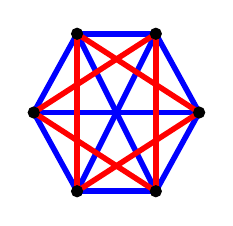
\begin{tikzpicture}
    \draw[line width=2pt, blue] (0,0) -- (1,0);
    \draw[line width=2pt, blue] (1,0) -- (1.55,1);
    \draw[line width=2pt, blue] (1.55,1) -- (1,2);
    \draw[line width=2pt, blue] (1,2) -- (0,2);
    \draw[line width=2pt, blue] (0,2) -- (-0.55,1);
    \draw[line width=2pt, blue] (-0.55,1) -- (0,0);
    \draw[line width=2pt, blue] (0,0) -- (1,2);
    \draw[line width=2pt, blue] (1.55,1) -- (-0.55,1);
    \draw[line width=2pt, blue] (1,0) -- (0,2);
    \draw[line width=2pt, red] (0,0) -- (0,2);
    \draw[line width=2pt, red] (1,0) -- (1,2);
    \draw[line width=2pt, red] (1,0) -- (-0.55,1);
    \draw[line width=2pt, red] (1.55,1) -- (0,2);
    \draw[line width=2pt, red] (1,2) -- (-0.55,1);
    \draw[line width=2pt, red] (0,0) -- (1.55,1);

    \filldraw (0,0) circle (2pt);
    \filldraw (1,0) circle (2pt);
    \filldraw (-0.55,1) circle (2pt);
    \filldraw (1.55,1) circle (2pt);
    \filldraw (0,2) circle (2pt);
    \filldraw (1,2) circle (2pt);

\end{tikzpicture}
\caption{An arbitrary 2-colouring of $K_6$}
\end{center}
\end{figure}

This graph describes a situation in which we have two disjoint sets of 3 people
which mutually do not know each other, illustrated by the two blue triangle which
lie within the graph. Since every point of the graph is connected to every other
point if the graph, we say it is $complete$, and we denote the graph
$K_n$, where n is the number of the vertices of the graph. We now give
the definition of a subgraph.\\

We can now ask a question which lies at the heart of Ramsey theory: Given positive
integers $s$ and $t$, can we always find a large enough group of people
such that $s$ mutually know each other, and $t$ do not? the answer
is yes, and I shall now phrase this using the graph theoretic language we have just established:

\begin{theorem}[Ramsey's theorem for graphs]

\end{theorem}


